\subsection{Persiapan Pengujian}
Pada proses pengujian, terdapat tiga lingkungan pengujian yang digunakan untuk menguji sistem \textit{remote deployment}. Ketiga lingkungan tersebut yaitu kubernetes \textit{cluster} lokal, kubernetes \textit{cluster} yang terdapat di \textit{Cloud (GCP)}, serta \textit{cluster} pada RaspberryPi. Ketiga \textit{cluster} ini memiliki jumlah node yang berbeda sesuai dengan penjelasan pada \ref{subsec:batasan-pengujian}.

\subsubsection{Kubernetes Lokal}
Untuk pengujian pada kubernetes lokal, dilakukan pembuatan \textit{cluster} dengan kakas kind untuk membuat cluster yang bernama \textit{testing-cluster-two-nodes} yang memiliki 2 node. Konfigurasi pembuatan sama seperti konfigurasi pada bagian \ref{subsec:persiapan-kubernetes-cluster} hanya saja jumlah nodes yang digunakan yaitu 2.
Karena nodes berjumlah dua maka terdapat 1 \textit{master nodes} dan 1 \textit{slave} node pada \textit{cluster}. Konfigurasi pembuatan cluster dapat dilihat pada gambar \ref{fig:kubernetes-lokal-config-testing}.

\begin{figure}[ht]
  \centering
  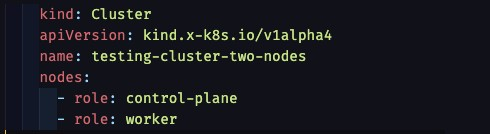
\includegraphics[width=1\textwidth]{resources/chapter-4/pengujian/kubernetes-lokal-config.jpg}
  \caption{Konfigurasi Pembuatan \textit{Kubernetes Testing Cluster} Dengan Kakas \textit{Kind}}
  \label{fig:kubernetes-lokal-config-testing}
\end{figure}

Setelah itu jalankan perintah "kind create cluster --config testing-cluster.yaml" untuk membuat \textit{cluster} pada \textit{docker}. Hasil dari perintahh ini yaitu tercipta dua buah \textit{container} pada \textit{docker} yang memiliki peran \textit{master} dan \textit{slave} seperti pada gambar \ref{fig:kubernetes-lokal-config-testing-result}.

\begin{figure}[ht]
  \centering
  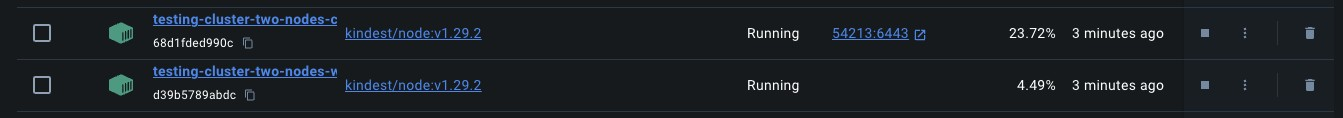
\includegraphics[width=1\textwidth]{resources/chapter-4/pengujian/kubernetes-lokal-config-result.jpg}
  \caption{Hasil \textit{Kubernetes Testing Cluster} pada \textit{Docker}}
  \label{fig:kubernetes-lokal-config-testing-result}
\end{figure}

\subsubsection{Kubernetes GCP}
\label{subsubsec:kubernetes-gcp}
Pada lingkungan ini dibuat dua buah \textit{compute engine (virtual machine)} pada \textit{GCP}. Masing masing dari \textit{virtual machine} berperan sebagai kubernetes \textit{cluster} yang bernama \textit{prod-cluster-example}.

\begin{enumerate}
  \item Buat dua \textit{virtual machine} pada \textit{compute engine GCP} dengan spesifikasi berikut. Hasil pembuatan \textit{virtual machine} dapat dilihat pada gambar \ref{fig:hasil-pembuatan-virtual-machine-gcp}
        \begin{enumerate}
          \item Ubuntu 24.04
          \item 2GB Memory
          \item 10GB Storage Persistent Disk
          \item 0.5 - 2Vcpu (1 shared core)
          \item Region Asia southeast2-c
        \end{enumerate}
  \item Membuat \textit{Firewall Rule} Untuk membuka port yang digunakan oleh Kubernetes. Untuk daftar opsi setiap port yang dibuka dapat dilihat pada gambar \ref{fig:daftar-kegunaan-port}. Untuk hasil pembuatan firewall dapat dilihat pada bagian \ref{fig:hasil-firewall-rule-pada-gcp}
  \item Konfigurasi \textit{gare-test-kubernetes-server} sebagai master nodes. Konfigurasi dilakukan dengan cara mengunduh instalasi dari k3s dengan perintah seperti pada gambar \ref{fig:instalasi-master-node-gcp}.
  \item Konfigurasi virutal machine lainnya yaitu \textit{gare-test-kubernetes-server-node} sebagai \textit{worker node}. Untuk meregistrasi \textit{node} ke dalam \textit{cluster} perlu adanya autentikasi untuk memasitikan hanya \textit{node} yang benar yang boleh masuk ke dalam \textit{cluster}. K3s memiliki token generator yang dapat digunakan untuk mencegah akses yang tidak diinginkan, registrasi token dapat dilihat pada gambar \ref{fig:pengambilan-token-registrasi-cluster}. Token tersebut digunakan untuk meregistrasi \textit{node} ini ke \textit{master} dengan \textit{public ip} node tersebut. Ilustrasi dapat dilihat pada gambar \ref{fig:instalasi-worker-node-gcp}.
  \item Ambil konfigurasi \textit{cluster} di \textit{master node} dan pindahkan ke lokasi \textit{server berjalan} untuk meregistrasi \textit{cluster} ke dalam sistem. Setelah melakukan kelima langkah ini \textit{cluster} sudah terintegrasi dengan sistem. Ilustrasi pemindahan konfigurasi dapat dilihat pada gambar \ref{fig:konfigurasi-cluster-master-node-gcp} dan \ref{fig:proses-pemindahan-konfigurasi-master-gcp}.
\end{enumerate}

\subsubsection{Kubernetes RaspberryPi}
Pada lingkungan ini dibuat cluster dengan dua nodes pada RaspberryPi. Cluster yang dibuat bernama cluster-raspi yang memiliki spesifikasi hardware RaspberryPi berikut.

\begin{enumerate}
  \item Master node menggunakan Raspberry Pi 3 Model B Rev 1.2 dengan 1GB RAM dan 4 CPU @ 1.2GHz dengan hostname masterpi. Informasi lebih lengkap dapat dilihat pada gambar \ref{fig:hostname-raspi-master-nodes} dan \ref{fig:spesifikasi-raspi-master-nodes}
  \item Worker node menggunakan Raspberry Pi 2 Model B Rev 1.1 dengan 1GB RAM dan 4 CPU @ 900MHz dengan hostname raspberrypi. Informasi lebih lengkap dapat dilihat pada gambar \ref{fig:hostname-raspi-worker-nodes} dan \ref{fig:spesifikasi-raspi-worker-nodes}
\end{enumerate}

Berikut merupakan tata cara pembuatan cluster kubernetes pada \textit{RaspberryPi}. Diasumsikan \textit{device} \textit{RaspberryPi} sudah terhubung ke dalam jaringan yang sama sehingga tidak perlu \textit{port forwarding} / \textit{public ip}.

\begin{enumerate}
  \item Konfigurasi \textit{hostname masterpi} sebagai master nodes. Perlu dilakukan konfigurasi tambahan untuk menambahkan cgroups pada raspberrypi karena secara default opsi ini \textit{disabled}. cgroups merupakan kepanjangan dari \textit{Control Groups} yang berfungsi sebagai \textit{resource management} pada linux dan digunakan dalam proses kontainerisasi. Selanjutnya mirip serperti konfigurasi pada bagian \ref{subsubsec:kubernetes-gcp}, perlu mengunduh instalasi dari k3s dengan perintah seperti pada gambar \ref{fig:instalasi-master-raspi-nodes}.
  \item Konfigurasi \textit{node} lainnya yaitu \textit{hostname raspberrypi} sebagai \textit{worker node}. Untuk meregistrasi \textit{node} ke dalam \textit{cluster} perlu adanya autentikasi untuk memasitikan hanya \textit{node} yang benar yang boleh masuk ke dalam \textit{cluster}. K3s memiliki token generator yang dapat digunakan untuk mencegah akses yang tidak diinginkan, registrasi token dapat dilihat pada gambar \ref{fig:raspi-master-gen-token}. Token tersebut digunakan untuk meregistrasi \textit{node} ini ke \textit{master} dengan \textit{ip local} node master. Ilustrasi dapat dilihat pada gambar \ref{fig:instalasi-worker-raspi-node}.
  \item Ambil konfigurasi \textit{cluster} di \textit{master node} dan pindahkan ke lokasi \textit{server berjalan} untuk meregistrasi \textit{cluster} ke dalam sistem. Setelah melakukan langkah ini \textit{cluster} sudah terintegrasi dengan sistem. Ilustrasi pemindahan konfigurasi dapat dilihat pada gambar \ref{fig:raspi-kube-config} dan \ref{fig:raspi-add-kubeconfig}.
\end{enumerate}